% author:   sam tenka
% change:   2022-05-23
% create:   2022-05-11

%==============================================================================
%====  0.  DOCUMENT SETTINGS  ================================================
%==============================================================================

%~~~~~~~~~~~~~~~~~~~~~~~~~~~~~~~~~~~~~~~~~~~~~~~~~~~~~~~~~~~~~~~~~~~~~~~~~~~~~~
%~~~~~~~~~~~~~  0.0. About this Exposition  ~~~~~~~~~~~~~~~~~~~~~~~~~~~~~~~~~~~

%---------------------  0.0.0. page geometry  ---------------------------------
\documentclass[11pt, justified]{tufte-book}
\geometry{
  left           = 0.90in, % left margin
  textwidth      = 4.95in, % main text block
  marginparsep   = 0.15in, % gutter between main text block and margin notes
  marginparwidth = 2.30in, % width of margin notes
                 % 0.20in  % width from margin to edge
}

%---------------------  0.0.1. math packages  ---------------------------------
\newcommand\hmmax{0} % to allow for more fonts 
\newcommand\bmmax{0} % to allow for more fonts
\usepackage{amsmath, amssymb, amsthm, mathtools}
\usepackage{bm}
\usepackage{euler}

\usepackage{array}   % for \newcolumntype macro
\newcolumntype{L}{>{$}l<{$}} % math-mode version of "l" column type
\newcolumntype{C}{>{$}c<{$}} % math-mode version of "c" column type
\newcolumntype{R}{>{$}r<{$}} % math-mode version of "r" column type

%---------------------  0.0.2. graphics packages  -----------------------------
\usepackage{graphicx, xcolor}
\usepackage{float, capt-of}

%---------------------  0.0.3. packages for fancy text  -----------------------
\usepackage{enumitem}\setlist{nosep}
\usepackage{listings}
\usepackage{xstring}
\usepackage{fontawesome5}

%---------------------  0.043. colors  ----------------------------------------
\definecolor{mblu}{rgb}{0.05, 0.35, 0.70} \newcommand{\blu}{\color{mblu}}
\definecolor{mbre}{rgb}{0.30, 0.45, 0.60} \newcommand{\bre}{\color{mbre}}
\definecolor{mbro}{rgb}{0.60, 0.05, 0.05} \newcommand{\bro}{\color{mbro}}
\definecolor{mcya}{rgb}{0.10, 0.45, 0.45} \newcommand{\cya}{\color{mcya}}
\definecolor{mgre}{rgb}{0.55, 0.55, 0.50} \newcommand{\gre}{\color{mgre}}
\definecolor{mgrn}{rgb}{0.15, 0.65, 0.05} \newcommand{\grn}{\color{mgrn}}
\definecolor{mred}{rgb}{0.90, 0.05, 0.05} \newcommand{\red}{\color{mred}}

%~~~~~~~~~~~~~~~~~~~~~~~~~~~~~~~~~~~~~~~~~~~~~~~~~~~~~~~~~~~~~~~~~~~~~~~~~~~~~~
%~~~~~~~~~~~~~  0.1. Headers and References  ~~~~~~~~~~~~~~~~~~~~~~~~~~~~~~~~~~

%---------------------  0.1.0. intra-document references  ---------------------
\newcommand{\offour}[1]{
    {\tiny \raisebox{0.04cm}{\scalebox{0.9}{$\substack{
        \IfSubStr{#1}{0}{{\blacksquare}}{\square}   
        \IfSubStr{#1}{1}{{\blacksquare}}{\square} \\ 
        \IfSubStr{#1}{2}{{\blacksquare}}{\square}   
        \IfSubStr{#1}{3}{{\blacksquare}}{\square}   
    }$}}}%
}

\newcommand{\offourline}[1]{
    {\tiny \raisebox{0.04cm}{\scalebox{0.9}{$\substack{
        \IfSubStr{#1}{0}{{\blacksquare}}{\square}   
        \IfSubStr{#1}{1}{{\blacksquare}}{\square}
        \IfSubStr{#1}{2}{{\blacksquare}}{\square}   
        \IfSubStr{#1}{3}{{\blacksquare}}{\square}   
    }$}}}%
}
\newcommand{\notesam}[1]{{\blu \textsf{#1}}}
\newcommand{\attn}[1]{{\bro \textsf{#1}}}
\newcommand{\attnsam}[1]{{\red \textsf{#1}}}

\newcommand{\blarr}{\hspace{-0.15cm}${\bro \leftarrow}\,$}
\newcommand{\bcirc}{${\bro ^\circ}$}

\newcounter{footprintssofar}
\setcounter{footprintssofar}{90}
\newcommand{\plainfootprint}{{\bro \rotatebox{\value{footprintssofar}}{\faIcon{shoe-prints}}}\setcounter{footprintssofar}{\value{footprintssofar}+30} }
\newcommand{\footprint}{\marginnote{\plainfootprint} }

%---------------------  0.1.1. table of contents helpers  ---------------------
\newcommand{\phdot}{\phantom{.}}

%---------------------  0.1.2. section headers  -------------------------------
\newcommand{\samtitle} [1]{
  \par\noindent{\Huge \sf \blu #1}
  \vspace{0.4cm}
}

\newcommand{\samquote} [2]{
    \marginnote[-0.4cm]{\begin{flushright}
    \scriptsize
        \gre {\it #1} \\ --- #2
    \end{flushright}}
}

\newcommand{\samsection} [1]{
  \vspace{0.5cm}
  \par\noindent{\LARGE \sf \blu #1}
  \vspace{0.1cm}\par
}

\newcommand{\samsubsection}[1]{
  \vspace{0.3cm}
  \par\noindent{\Large \sf \bre #1}
  \vspace{0.1cm}\par
}

\newcommand{\samsubsubsection}[1]{
   \vspace{0.1cm}
   \par\noindent{\hspace{-2cm}\normalsize \sc \gre #1} ---
}

%---------------------  0.1.3. clear the bibliography's header  ---------------
\usepackage{etoolbox}
\patchcmd{\thebibliography}{\section*{\refname}}{}{}{}

%~~~~~~~~~~~~~~~~~~~~~~~~~~~~~~~~~~~~~~~~~~~~~~~~~~~~~~~~~~~~~~~~~~~~~~~~~~~~~~
%~~~~~~~~~~~~~  0.2. Math Symbols and Blocks  ~~~~~~~~~~~~~~~~~~~~~~~~~~~~~~~~~

%---------------------  0.2.0. general math operators  ------------------------
\newcommand{\scirc}{\mathrel{\mathsmaller{\mathsmaller{\mathsmaller{\circ}}}}}
\newcommand{\cmop}[2]{{(#1\!\to\!#2)}}

%---------------------  0.2.1. probability symbols  ---------------------------
\newcommand{\KL}{\text{KL}}
\newcommand{\EN}{\text{H}}
\newcommand{\note}[1]{{\blu \textsf{#1}}}

%---------------------  0.2.2. losses averaged in various ways  ---------------
\newcommand{\Ein}  {\text{trn}_{\sS}}
\newcommand{\Einb} {\text{trn}_{\check\sS}}
\newcommand{\Einc} {\text{trn}_{\sS\sqcup \check\sS}}
\newcommand{\Egap} {\text{gap}_{\sS}}
\newcommand{\Eout} {\text{tst}}

%---------------------  0.2.3. double-struck and caligraphic upper letters  ---
\newcommand{\Aa}{\mathbb{A}}\newcommand{\aA}{\mathcal{A}}
\newcommand{\Bb}{\mathbb{B}}\newcommand{\bB}{\mathcal{B}}
\newcommand{\Cc}{\mathbb{C}}\newcommand{\cC}{\mathcal{C}}
\newcommand{\Dd}{\mathbb{D}}\newcommand{\dD}{\mathcal{D}}
\newcommand{\Ee}{\mathbb{E}}\newcommand{\eE}{\mathcal{E}}
\newcommand{\Ff}{\mathbb{F}}\newcommand{\fF}{\mathcal{F}}
\newcommand{\Gg}{\mathbb{G}}\newcommand{\gG}{\mathcal{G}}
\newcommand{\Hh}{\mathbb{H}}\newcommand{\hH}{\mathcal{H}}
\newcommand{\Ii}{\mathbb{I}}\newcommand{\iI}{\mathcal{I}}
\newcommand{\Jj}{\mathbb{J}}\newcommand{\jJ}{\mathcal{J}}
\newcommand{\Kk}{\mathbb{K}}\newcommand{\kK}{\mathcal{K}}
\newcommand{\Ll}{\mathbb{L}}\newcommand{\lL}{\mathcal{L}}
\newcommand{\Mm}{\mathbb{M}}\newcommand{\mM}{\mathcal{M}}
\newcommand{\Nn}{\mathbb{N}}\newcommand{\nN}{\mathcal{N}}
\newcommand{\Oo}{\mathbb{O}}\newcommand{\oO}{\mathcal{O}}
\newcommand{\Pp}{\mathbb{P}}\newcommand{\pP}{\mathcal{P}}
\newcommand{\Qq}{\mathbb{Q}}\newcommand{\qQ}{\mathcal{Q}}
\newcommand{\Rr}{\mathbb{R}}\newcommand{\rR}{\mathcal{R}}
\newcommand{\Ss}{\mathbb{S}}\newcommand{\sS}{\mathcal{S}}
\newcommand{\Tt}{\mathbb{T}}\newcommand{\tT}{\mathcal{T}}
\newcommand{\Uu}{\mathbb{U}}\newcommand{\uU}{\mathcal{U}}
\newcommand{\Vv}{\mathbb{V}}\newcommand{\vV}{\mathcal{V}}
\newcommand{\Ww}{\mathbb{W}}\newcommand{\wW}{\mathcal{W}}
\newcommand{\Xx}{\mathbb{X}}\newcommand{\xX}{\mathcal{X}}
\newcommand{\Yy}{\mathbb{Y}}\newcommand{\yY}{\mathcal{Y}}
\newcommand{\Zz}{\mathbb{Z}}\newcommand{\zZ}{\mathcal{Z}}

%---------------------  0.2.4. sans serif and frak lower letters  -------------
\newcommand{\sfa}{\mathsf{a}}\newcommand{\fra}{\mathcal{a}}
\newcommand{\sfb}{\mathsf{b}}\newcommand{\frb}{\mathcal{b}}
\newcommand{\sfc}{\mathsf{c}}\newcommand{\frc}{\mathcal{c}}
\newcommand{\sfd}{\mathsf{d}}\newcommand{\frd}{\mathcal{d}}
\newcommand{\sfe}{\mathsf{e}}\newcommand{\fre}{\mathcal{e}}
\newcommand{\sff}{\mathsf{f}}\newcommand{\frf}{\mathcal{f}}
\newcommand{\sfg}{\mathsf{g}}\newcommand{\frg}{\mathcal{g}}
\newcommand{\sfh}{\mathsf{h}}\newcommand{\frh}{\mathcal{h}}
\newcommand{\sfi}{\mathsf{i}}\newcommand{\fri}{\mathcal{i}}
\newcommand{\sfj}{\mathsf{j}}\newcommand{\frj}{\mathcal{j}}
\newcommand{\sfk}{\mathsf{k}}\newcommand{\frk}{\mathcal{k}}
\newcommand{\sfl}{\mathsf{l}}\newcommand{\frl}{\mathcal{l}}
\newcommand{\sfm}{\mathsf{m}}\newcommand{\frm}{\mathcal{m}}
\newcommand{\sfn}{\mathsf{n}}\newcommand{\frn}{\mathcal{n}}
\newcommand{\sfo}{\mathsf{o}}\newcommand{\fro}{\mathcal{o}}
\newcommand{\sfp}{\mathsf{p}}\newcommand{\frp}{\mathcal{p}}
\newcommand{\sfq}{\mathsf{q}}\newcommand{\frq}{\mathcal{q}}
\newcommand{\sfr}{\mathsf{r}}\newcommand{\frr}{\mathcal{r}}
\newcommand{\sfs}{\mathsf{s}}\newcommand{\frs}{\mathcal{s}}
\newcommand{\sft}{\mathsf{t}}\newcommand{\frt}{\mathcal{t}}
\newcommand{\sfu}{\mathsf{u}}\newcommand{\fru}{\mathcal{u}}
\newcommand{\sfv}{\mathsf{v}}\newcommand{\frv}{\mathcal{v}}
\newcommand{\sfw}{\mathsf{w}}\newcommand{\frw}{\mathcal{w}}
\newcommand{\sfx}{\mathsf{x}}\newcommand{\frx}{\mathcal{x}}
\newcommand{\sfy}{\mathsf{y}}\newcommand{\fry}{\mathcal{y}}
\newcommand{\sfz}{\mathsf{z}}\newcommand{\frz}{\mathcal{z}}

%---------------------  0.2.5. math environments  -----------------------------
\newtheorem*{qst}{Question}
\newtheorem*{thm}{Theorem}
\newtheorem*{lem}{Lemma}
% ...
\theoremstyle{definition}
\newtheorem*{dfn}{Definition}

%==============================================================================
%=====  1.  PROLOGUE  =========================================================
%==============================================================================

\begin{document}
\samtitle{recitation 01 (optional 6.86x notes)}

      \marginnote{%
        %These notes overlap with what we'll cover in recitation.  But
        Recitation will have more coding practice and much less detail than
        these notes.  We'll skip whole sections of these notes during
        recitation.
        %
        Footprints --- \plainfootprint --- in these notes indicate roughly
        which points we will linger on during recitation.  Each footprint
        represents perhaps three to seven minutes of recitation time.  
        %
        %A recitation might have eighteen footprints.
      }

      \attn{You do not need to read these notes at all} to get an A
      in this course; conversely, \attn{you may not cite these notes} when
      solving homework or exams.
       
  \samsection{A. Prologue}

    \samsubsection{bird's eye view}
 
      \samsubsubsection{kinds of learning}
        How do we communicate patterns of desired behavior?  We can teach:\footprint
        \begin{description}
          \item[\textbf{by instruction}:  ]  ``to tell whether a mushroom is poisonous, first look at its gills...'' 
          \item[\textbf{by example}:      ]  ``here are six poisonous fungi; here, six safe ones.  see a pattern?''
          \item[\textbf{by reinforcement}:]  ``eat foraged mushrooms for a month; learn from getting sick.''
        \end{description}
        %
        Machine learning is the art of programming computers to learn from such
        sources.  We'll focus on the most important case: learning from
        examples.\bcirc\marginnote{%
          \blarr In Unit 5 of 6.86x, we'll see that learning by example is key to
          the other modes of learning.
        }

      \samsubsubsection{from examples to predictions}
        For us, a pattern of desired behavior is a function that for each given
        situation/prompt returns a favorable action/answer.\footprint
        %
        Our goal is to write a program that, from a list of $N$ examples of
        prompts and matching answers, determines an underlying pattern.  We
        consider our program a success if this pattern accurately predicts
        answers corresponding to new, unseen prompts.
        %
        We often define our program as a search, over some set $\hH$ of
        candidate patterns, to minimize some notion of ``discrepancy from the
        example data''.\footprint

        \begin{figure}[h]
          \vspace{-0.5cm}
          \par\noindent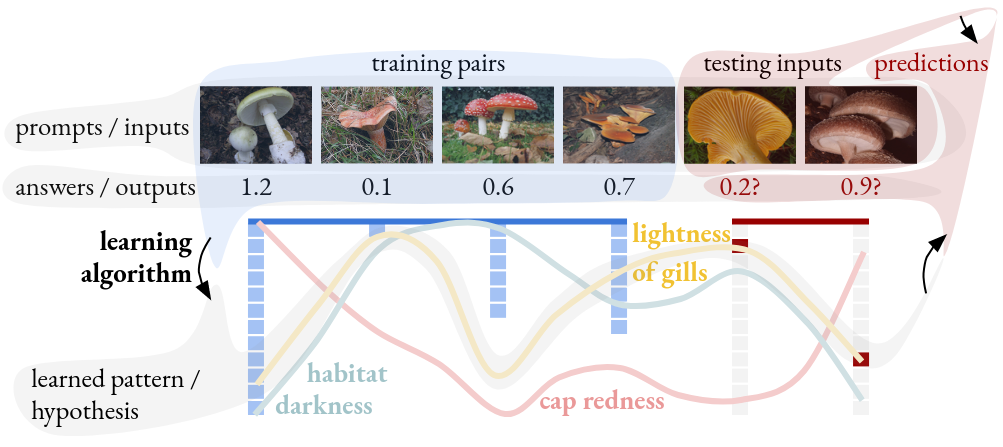
\includegraphics[width=\textwidth]{figures/supervised}\\
          \caption{%
            A program that learns to predict mushrooms' poison levels:
            %
            first takes a list of labeled mushrooms as input (blue blob);
            searches
            through candidate patterns (here, the wiggly curves labeled
            \texttt{lightness of gills}, \texttt{habitat darkness}, and
            \texttt{cap redness}); and returns the pattern that best fits the
            examples.
            %
            Evaluating this pattern on new mushrooms, we predict their poison
            levels (red blob). 
            %
            \par The three bold black arrows show the flow of data from
            training examples to a learned pattern; and from that pattern
            together with testing prompts to predictions.  
            %
            Part of specifying the learning program is specifying the set of candidate patterns to consider.
          }
          \vspace{-0.5cm}
        \end{figure}

        To save ink, say that $\xX$ is the set of possible prompts; $\yY$, of
        possible answers.\bcirc\marginnote{%
          \blarr If we like, we can now summarize the data flow in symbols.  A
          pattern is a function of type $\xX\to\yY$.  And we can model the
          examples from which our program learns as a list of type $(\xX\times
          \yY)^N$.  Then a program that learns from examples has type:
          $$
            \lL : (\xX\times \yY)^N \to (\xX\to \yY)
          $$
          Once we allow uncertainty by letting patterns map to \emph{probability
          distributions} over answers, the type will change to:
          $$
            \lL : (\xX\times \yY)^N \to (\xX\to \text{DistributionsOn}(\yY))
          $$
        }
        In the mushrooms example, $\xX$ contains all
        conceivable mushrooms and $\yY$ contains all conceivable poison
        levels (perhaps all the non-negative real numbers).

      \samsubsubsection{supervised learning}
        We'll soon allow uncertainty by letting patterns map to \emph{probability
        distributions} over answers.
        %
        Even if the prompt is always the same --- say, ``produce a beautiful
        melody'', we may seek to understand the complicated distribution over
        answers.  We might regard our program a success if it can
        generate a variety of good answers.
        %
        So-called \textbf{unsupervised learning} focuses in that way on output
        structure.  By contrast, \textbf{supervised learning} (our subject in
        Unit 1), focuses on the input-output relation; it's interesting when
        the space of prompts is large.\footprint
        %

    \newpage
    \samsubsection{a tiny example: handwritten digit classification}
      \samsubsubsection{meeting the data}
        $\xX = \{\text{grayscale~}28\!\times\!28\text{-pixel images}\}$;
        $\yY=\{{\cya{1}},{\red{9}}\}$.  Each datum $(x,y)$ arises as follows:
        we randomly choose a digit $y\in \yY$, ask a human to write that digit
        in pen, and then photograph their writing to produce $x\in\xX$.\footprint
        %

        \vspace{-0.25cm}
        \begin{figure}
            \centering
          \begin{tabular}{c}
\includegraphics[width=0.75cm]{example-mnist/mnist-trn-00}\\$\red{9}$\\
\includegraphics[width=0.75cm]{example-mnist/mnist-trn-10}\\$\cya{1}$\end{tabular}%
          \begin{tabular}{c}
\includegraphics[width=0.75cm]{example-mnist/mnist-trn-01}\\$\cya{1}$\\
\includegraphics[width=0.75cm]{example-mnist/mnist-trn-11}\\$\red{9}$\end{tabular}%
          \begin{tabular}{c}
\includegraphics[width=0.75cm]{example-mnist/mnist-trn-02}\\$\red{9}$\\
\includegraphics[width=0.75cm]{example-mnist/mnist-trn-12}\\$\cya{1}$\end{tabular}%
          \begin{tabular}{c}
\includegraphics[width=0.75cm]{example-mnist/mnist-trn-03}\\$\red{9}$\\
\includegraphics[width=0.75cm]{example-mnist/mnist-trn-13}\\$\cya{1}$\end{tabular}%
          \begin{tabular}{c}
\includegraphics[width=0.75cm]{example-mnist/mnist-trn-04}\\$\cya{1}$\\
\includegraphics[width=0.75cm]{example-mnist/mnist-trn-14}\\$\red{9}$\end{tabular}%
          \begin{tabular}{c}
\includegraphics[width=0.75cm]{example-mnist/mnist-trn-05}\\$\red{9}$\\
\includegraphics[width=0.75cm]{example-mnist/mnist-trn-15}\\$\red{9}$\end{tabular}%
          \begin{tabular}{c}
\includegraphics[width=0.75cm]{example-mnist/mnist-trn-06}\\$\red{9}$\\
\includegraphics[width=0.75cm]{example-mnist/mnist-trn-16}\\$\red{9}$\end{tabular}%
          \begin{tabular}{c}
\includegraphics[width=0.75cm]{example-mnist/mnist-trn-07}\\$\red{9}$\\
\includegraphics[width=0.75cm]{example-mnist/mnist-trn-17}\\$\cya{1}$\end{tabular}%
          \begin{tabular}{c}
\includegraphics[width=0.75cm]{example-mnist/mnist-trn-08}\\$\cya{1}$\\
\includegraphics[width=0.75cm]{example-mnist/mnist-trn-18}\\$\red{9}$\end{tabular}%
          \begin{tabular}{c}
\includegraphics[width=0.75cm]{example-mnist/mnist-trn-09}\\$\red{9}$\\
\includegraphics[width=0.75cm]{example-mnist/mnist-trn-19}\\$\cya{1}$\end{tabular}%
          \caption{
            Twenty example pairs.  Each photo $x$ is a $28\times 28$ grid of
            numbers representing pixel intensities.  The light gray background
            has intensity $0.0$; the blackest pixels, intensity $1.0$.  Below
            each photo $x$ we display the corresponding label $y$:
            either $y= {\cya{1}}$ or
            $y={\red{9}}$.
            %
            We'll adhere to this color code throughout this tiny example.
          }
        \end{figure}

        \footprint
        As part of getting to know the data, it's worth taking a moment to
        think about how we would go about hand-coding a digit classifier.  The
        challenge is to complete the pseudocode
        %
        ``\texttt{if (?)\ then predict y=9 else predict y=1}''.
        %
        Well, ${\red{9}}$s tend to have more ink than than ${\cya{1}}$s ---
        should \texttt{(?)}\ threshold by the photo's darkness?
        %
        Or: ${\cya{1}}$s tend to be wider than ${\red{9}}$s --- should 
        \texttt{(?)}\ threshold by the photo's dark part's width?

        To make this precise, let's define a photo's \emph{darkness} as its
        average pixel darkness; its \emph{width} as the standard deviation of
        the column index of its dark pixels.  For convenience let's normalize
        both width and darkness to have max possible value $1.0$.  Such
        functions from inputs in $\xX$ to numbers are called
        \textbf{features}.\footprint

        \begin{lstlisting}[language=Python, basicstyle=\footnotesize\ttfamily]
          SIDE = 28
          def darkness(x):
            return np.mean(np.mean(x))
          def width(x):
            return np.std([col for col in range(SIDE)
                               for row in range(SIDE)
                               if 0.5 < x[row][col]  ])/(SIDE/2.0) 
        \end{lstlisting}

        So we can threshold by darkness or by width.  But this isn't very
        satisfying, since sometimes there are especially dark ${\cya{1}}$s or
        wide ${\red{9}}$s. 
        %
        We thus arrive at the idea of using \emph{both} features: ${\red{9}}$s
        are darker than ${\cya{1}}$s \emph{even relative to their
        width}.  So we might write something like
        \texttt{2*darkness(x)-width(x)>0} for\bcirc\marginnote{%
          \blarr That factor of
          $2$ comes from our observation that darkness and tends to be $0.15$
          while width tends to be around $0.30$.
        } our condition.

        \begin{lstlisting}[language=Python, basicstyle=\footnotesize\ttfamily]
          def hand_coded_predict(x):
            return 9 if 2*darkness(x)-width(x)>0 else 1
        \end{lstlisting}

        \noindent
        \attn{Exercise:} {Beyond width and darkness, what features do you think
        might help us to separate digits $1$ from $9$?
        How about $0$ from $9$?}\footprint

    %\newpage
      \samsubsubsection{candidate patterns}
        We can generalize the hand-coded hypothesis from the previous passage
        to other coefficients besides $1\cdot \text{width}(x) -
        2\cdot\text{darkness}(x)$.  We let our set $\hH$ of candidate patterns
        contain all ``linear hypotheses'' $f_{a,b}$ defined by:\footprint
        $$
          f_{a,b}(x) = {\red{9}} \text{~~if~~} a\cdot\text{darkness}(x) + b\cdot\text{width}(x) > 0 \text{~~else~~} {\cya{1}}
        $$ 
        Each $f_{a,b}$ makes predictions of $y$s given $x$s.  As we change $a$
        and $b$, we get different predictors, some more accurate than others.

        \begin{lstlisting}[language=Python, basicstyle=\footnotesize\ttfamily]
          def predict(x,a,b):
            return 9 if a*width(x) + b*darkness(x) > 0 else 1
        \end{lstlisting}

        \noindent
        \attn{Exercise:} {how do $\offourline{0}$'s $3$ straight lines and
        $\offourline{1}$'s $3$ marked points correspond?}\footprint

      \samsubsubsection{optimization}
        Let's write a program $\lL$ that given a list of \emph{training
        examples} produces a hypothesis in $h \in \hH$ that helps us predict
        the labels $y$ of yet-unseen photos $x$ (\emph{testing examples}).
        Insofar as training data is representative of testing data, it's
        sensible to return a $h\in \hH$ that correctly classifies maximally
        many training examples.\footprint
        %
        To do this, let's make $\lL$ loop over all integer pairs $(a,b)$ in
        $[-99,+99]$:  %to minimize the number of misclassified training examples. 
        \begin{lstlisting}[language=Python, basicstyle=\footnotesize\ttfamily]
          def accuracy_on(examples,a,b):
            return sum(1.0 for x,y in examples if predict(x,a,b)==y)/len(examples)
          def best_hypothesis():
            return max((accuracy_on(training_data, a, b), (a,b))
                       for a in range(-99,100) 
                       for b in range(-99,100))
        \end{lstlisting}

        \begin{figure}[h]
            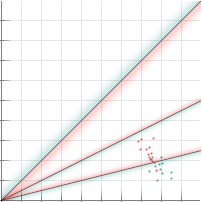
\includegraphics[width=0.24\textwidth]{example-mnist/train.png}%
            \hspace{0.005\textwidth}%
            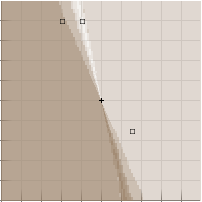
\includegraphics[width=0.24\textwidth]{example-mnist/train-scat.png}%
            \hspace{0.02\textwidth}%
            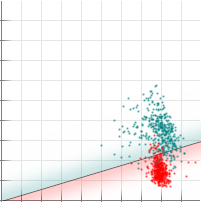
\includegraphics[width=0.24\textwidth]{example-mnist/test.png}%
            \hspace{0.005\textwidth}%
            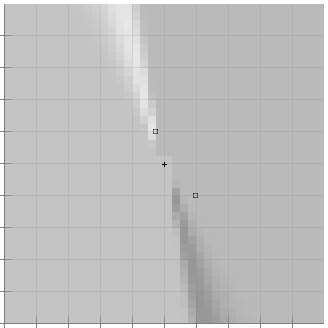
\includegraphics[width=0.24\textwidth]{example-mnist/test-scat.png}
            %
            \caption{
              \textbf{Training
              ($\protect\offourline{01}$) and testing
              ($\protect\offourline{23}$).}
              %
              $3$ hypotheses classify
              training data in the darkness-width plane ($\protect\offourline{0}$).
              %
              Each point in the $(a,b)$ plane ($\protect\offourline{1}$) represents
              a hypothesis; we shade them by the fraction of training
              data they misclassify: darker means less accurate.
              %
              Panes $\protect\offourline{23}$ show the same for
              \emph{testing} data.
              %
              $\protect\offourline{02}$'s axes range $[0, 0.5]$.
              $\protect\offourline{13}$'s axes range $[-99,+99]$. 
            }
        \end{figure}


        When we feed $N=25$ training examples to $\lL$, it produces
        $(a,b)=(80,-20)$ as a minimizer of training-error.  with $5\%$ of training examples
        misclassified.\footprint However, the same hypothesis %$(a,b)=(-20,6)$
        misclassifies a greater fraction --- $8\%$ --- of fresh testing
        examples.

        \noindent
        \attn{Exercise:} {visualize $f_{a,b}$'s error on $N=1$ example as a 
        function of $(a,b)$.}\footprint

      \samsubsubsection{error analysis}
        We got optimization error
        $\approx 0$ (albeit by \emph{unscalable brute-force}).  So
        approximation error $\approx \Ein \approx 5\%$.  Indeed, our straight
        lines are \emph{too simple}: width and darkness lose useful information
        and the ``true'' boundary looks curved (see $\offourline{0}$'s
        curve).\footprint
        %
        The testing error $\Eout \approx 8\%$ exceeds $\Ein$: we suffer
        \emph{generalization error}.
        %% actually approx error should be measured on the train set, which ain't that bad
        %
        In 6.86x we'll address all three italicized issues.

    %\newpage
    \samsubsection{supervised learning framework}
      \samsubsubsection{formalism}
        Draw training examples $\sS : (\xX\times \yY)^N$ %a list of examples
        from nature's distribution $\dD$ on $\xX\times \yY$.  A pattern
        $f:\xX\to \yY$ has \textbf{training error}
        $
           \Ein(f) = \Pp_{(x,y)\sim \red{\sS}}[f(x)\neq y] 
        $, an average over examples; and \textbf{testing error}
        $
           \Eout(f) = \Pp_{(x,y)\sim \red{\dD}}[f(x)\neq y] 
        $, an average over nature.  A \emph{learning program} is a function 
        $
            \lL : (\xX\times \yY)^N \to (\xX\to \yY)
        $; we want to design $\lL$ so that it maps typical $\sS$s to $f$s with
        low $\Eout(f)$.\marginnote{%
          %  TODO: mention extereme class-imbalance and bayesian *decision* theory 
        }

      \samsubsubsection{learning error}
        As in the previous subsection's tiny example,  
        we often define
        $\lL$ to roughly
        minimize $\Ein$ over a
        set $\hH \subseteq (\xX\to \yY)$ of candidate patterns.  Then $\Eout$
        decomposes
        into the failures
        of
        $\Ein$ to estimate $\Eout$ (generalization),
        of
        $\lL$ to minimize $\Ein$ (optimization), and 
        of
        $\hH$ to contain
        nature's
        truth (approximation): 
        \newcommand{\minf}[1]{{\inf}_{\hH}}
        \begin{align*}
            \Eout(\lL(\sS)) 
            =~&\Eout(\lL(\sS))      &-\,\,\,&      \Ein(\lL(\sS)) &~\}~& \text{\textbf{generalization} error} \\
            +~&\Ein(\lL(\sS))       &-\,\,\,& \minf{\hH}(\Ein(f)) &~\}~& \text{\textbf{optimization} error} \\
            +~&\minf{\hH}(\Ein(f))  &       &                     &~\}~& \text{\textbf{approximation} error}  
        \end{align*}
        These terms are in tension.  For example, as $\hH$ grows, the
        approx.\ error may decrease while the gen.\ error may
        increase --- this is the ``\textbf{bias-variance} tradeoff''.

        \noindent
        \attn{Exercise:} {why is generalization error usually positive?}\footprint

        %In the previous subsection, we got optimization error
        %$\approx 0$ (albeit by \emph{unscalable brute-force}).  So
        %approximation error $\approx \Ein \approx 5\%$.  Indeed, our straight
        %lines are \emph{too simple}: width and darkness lose useful information
        %and the ``true'' boundary looks curved (see $\offourline{0}$'s
        %curve).\footprint
        %%
        %The testing error $\Eout \approx 8\%$ exceeds $\Ein$: we suffer
        %\emph{generalization error}.
        %%% actually approx error should be measured on the train set, which ain't that bad
        %%
        %In 6.86x we'll address all three italicized issues.

      \samsubsubsection{workflow: framing}
        \emph{Framing} is about knowing our data and knowing what problem we
        want it to help solve.  Framing includes \emph{factorizing} a complex
        prediction problem into simple classification and regression problems;
        preparing and \emph{splitting} the consequent example pairs into
        training, development, and testing sets, and and \emph{visualizing} the
        training data to weigh our intuitions. 

      \samsubsubsection{workflow: modeling}
        \emph{Modeling} is about presenting our data in a way that is easy to
        digest for the computer --- in a way that easily found patterns are
        intuitively likely to be accurate. 
        %
        This is the key stage where we will inject our \emph{domain knowledge}
        --- that is, our human experience and intuition about which factors
        are likely to help with prediction.
        %
        Modeling includes \emph{featurizing} our inputs and \emph{regularizing}

        by choosing a class of \emph{priors} and symmetries.

      \samsubsubsection{workflow: training}
        \emph{Training} is about getting the computer to digest the data we've
        given it.  Under the hood, the computer will try a zillion candidate
        patterns until it hits upon one that explains the examples relatively
        well.  Above, we used brute force search; soon we'll learn more
        efficient approximate algorithms such as \emph{gradient descent}. 
        Training also involves \emph{model selection}: selecting from several
        qualitatively different models one that best predicts the development
        set.

      \samsubsubsection{workflow: harvesting}
        \emph{Harvesting} is about doing stuff with the pattern the computer
        settled on after it tried a zillion candidates.  We can derive insights
        from the pattern itself (which factors ended up being most important?)
        and we can predict outputs corresponding to fresh inputs.
        %
        Qualifying both applications is the pattern's quality.  To assess this,
        we measure its accuracy on our held-out testing data.

%==============================================================================
%=====  2.  LINEAR MODELS  ====================================================
%==============================================================================

  \newpage
  \samsection{B. linear models: the basics}
    \samsubsection{linear approximations} 
      \samquote{
        He had bought a large map representing the sea, \\
        Without the least vestige of land: \\
        And the crew were much pleased when they found it to be \\
        A map they could all understand.
      }{charles dodgson}
      \samsubsubsection{featurization}  % as an art of 
        As in the prologue, we represent our input $x$ as a fixed-length list
        of numbers so that we can treat $x$ with math. % \footprint
        There,
        we represented each photograph by $2$ numbers: width and
        darkness.  We could instead have represented each photograph by $784$
        numbers, one for the brightness at each of the $28\cdot 28=784$ many
        pixels.  Or by $10$ numbers, each measuring the overlap of $x$'s
        ink with that of ``representative'' photos of the digits $0$ through $9$.

        When we choose how to represent $x$ by a list of numbers, %\footprint
        we're
        choosing a \textbf{featurization}.  We call each number a ``feature''.
        For example, width and darkness are two features.

        %``width'' and ``darkness'' are \emph{features}: maps $\xX\to \Rr$ used
        %to pre-process $x$s.

        \attnsam{TODO: mention one-hot, etc}
        \attnsam{TODO: mention LOWRANK for multiregression? (relevant to futrure intermezzo?}
        %
        There are lots of interesting featurizations, each making different
        patterns easier to learn.  So we judge a featurization with respect to
        the kinds of patterns we use it to learn. %\footprint
        \attnsam{TODO: graphic of separability; and how projection can reduce it}
        Learning usually happens
        more accurately, robustly, and interpretably when our featurization is
        abstract (no irrelevant details) but complete (all relevant details),
        compressed (hard to predict one feature from the others) but accessible
        (easy to compute interesting properties).



      \samsubsubsection{geometry of feature-space} % pictures!

        Caution: a feature $A(\sfx)$ that is statistically independent from
        $\sfy$ may still be relevant for predicting $\sfy$.\marginnote{%
          Example.  Consider the uniform distribution on the four corners of a
          tetrahedron embedded within the corners of a cube \attnsam{TODO:
          graphic}.  The three spatial coordinates give three bit-valued random
          variables.  Any two of these variables are independent.  But the
          three together are dependent.
          \attnsam{TODO: also do a decision boundary (simpsons style) graph
          illustrating this phenomenon}
        }
        For example, if
        $A, B$ are two features, it is possible that $A(\sfx), \sfy$ are
        independent and that $B(\sfx), \sfy$ are independent and yet
        $A(\sfx),B(\sfx), \sfy$ are \emph{dependent}!

        \attnsam{TODO: example featurization (e.g. MNIST again?)}

        \attnsam{TODO: projectivization (say this foreshadows kernel discussion?)}

        Now say we've decided on a \textbf{featurization} of our input
        data $x$.
        $$
          f_{a,b}(x) = ~0 \text{~~if~~} a\cdot \text{width}(x) + b\cdot\text{darkness}(x) < 0 \text{~~else~~} 1 
        $$ 

        \attnsam{Illustrate `averaging' of good features vs `correction' of one feature by another (how much a feature correlates with error)}

      \samsubsubsection{linear algebra} % vectors and co-vectors
        Linear algebra is the part of geometry that focuses on %the notions of
        when a point is the origin, when a `line' is a straight, and when two
        straight lines are parallel.
        %
        Linear algebra thus helps us deal with the preceding pictures\marginnote{%
          $\leftarrow$ It is important to \attn{thoroughly understand these
          basics} of linear algebra.  Please see \S G.2 for further discussion
          of these basics. 
        }
        mathematically.  The concept of `straight lines' gives a simple,
        flexible model for extrapolation from known points to unknown points.
        That is intuitively why linear algebra will be crucial at every stage
        of 6.86x.

        The elements of linear algebra are \textbf{column vectors} and
        \textbf{row vectors}.  \attnsam{FILL IN}
        Though we represent the two similarly in a
        computer's memory, they have different geometric meanings.
        We save 
        much anguish by remembering the difference.  \attnsam{FILL IN}

        \attnsam{FILL IN LINEAR DECISION BOUNDARY! (remark on featurization and
        argmax nonlinearities)}

        We may \textbf{evaluate} a row vector on a column vector.  \attnsam{FILL
        IN} A \textbf{dot product} is a way of translating between row and
        column vectors.  \attnsam{FILL IN: DISCUSS GENERALIZATION; (DISCUSS ANGLE, TOO)}

      \samsubsubsection{richer outputs}%larger $\yY$s} % $k$-ary classification; regression; probabilities
        We've learned how to construct a set $\hH$ of candidate patterns 
        $$
          f_{\vec w}(\vec x) = \text{threshold}(\vec w\cdot \vec x) 
        $$
        that map (a featurization of) a prompt $\vec x$ to a binary answer $y=0$ or $y=1$.

        What if we're interested in predicting a richer kind of $y$?  For
        example, maybe there are $k$ many possible values for $y$ instead of
        just $2$.  Or maybe there are infinitely many possible values --- say,
        if $y$ is a real number or a length-$l$ list of real numbers.  Or maybe we want the added nuance of
        predicting probabilities, so that $f$ might output ``20\% chance of
        label $y=0$ and 80\% chance of label $y=1$'' instead of just ``$y=1$''.

        I'll write formulas and then explain.
        $$
          f_{\vec w_i : 0\leq i < k}(\vec x) = \text{argmax}_i(\vec w_i\cdot \vec x) 
        $$
        $$
          f_{\vec w}(\vec x) = \vec w \cdot \vec x
        $$
        \attnsam{TODO: add multi-output regression?}
        $$
          f_{\vec w_i  : 0\leq i < k}(\vec x) = \text{normalize}(\exp(\vec w_i \cdot \vec x) : 0\leq i < k)
        $$
        \attnsam{TODO: interpret}

        \attnsam{TODO: discuss measures of goodness!}

        \attnsam{TODO: talk about structured (trees/sequences/etc) output!}


    \newpage
    \samsubsection{iterative optimization} 
      \samquote{
        Hey Jude, don't make it bad \\
        Take a sad song and make it better \\
        Remember to let her under your skin \\
        Then you'll begin to make it \\
        Better, better, better, better, better, better, ...
      }{paul mccartney, john lennon}

      \samsubsubsection{(stochastic) gradient descent}
        We have a collection $\hH$ of candidate patterns together with a
        function $1-\Ein$ that tells us how good a candidate is.\marginnote{%
          $\leftarrow$ We view $1-\Ein$ as an estimate of our actual notion of ``good'': $1-\Eout$.
        }
        %
        In \S A we found a nearly best candidate by brute-force search over all of
        $\hH$; this doesn't scale to the general case, where $\hH$ is
        intractably large.
        %
        So: \emph{what's a faster algorithm to find a nearly best candidate?}

        A common idea is to start arbitrarily with some $h_0\in \hH$ and
        repeatedly improve to get $h_1, h_2, \cdots$.  Two questions are:
        \emph{how do we select $h_{t+1}$ in terms of $h_t$}?  And \emph{how do
        we know when to stop}?  We'll discuss termination conditions later
        --- for now, let's agree to stop at $h_{10000}$.   

        As for selecting a next candidate, we'd like to use more detailed
        information on $h_t$'s inadequacies to inform our proposal $h_{t+1}$.
        Intuitively, if $h_t$ misclassifies a particular $(x_n, y_n) \in \sS$,
        then we'd like $h_{t+1}$ to be like $h_t$ but nudged a bit in the
        direction of accurately classifying $(x_n, y_n)$.

        %
        \attnsam{FILL IN FOR PROBABILITIES (LOGISTIC) MODEL} 

        This is the idea of \textbf{gradient descent}.
        \attnsam{MOTIVATE AND GIVE PSEUDOCODE FOR STOCHASTIC GD} 
        
      \samsubsubsection{logistic models} %``soft''

        \attnsam{mention convexity and convergence?}

      %\samsubsubsection{perceptrons} %as constrained logistic regression; ``hard''
        We get a historically crucial and intuition-pumping algorithm when we
        do logistic regression in the limit of low temperatures.

        \attnsam{mention convergence?}
        \attnsam{show trajectory in weight space over time -- see how certainty degree of freedom is no longer redundant? (``markov'')}

      \samsubsubsection{humble models}
        %Logistic ain't the only way to go.
        Let's generalize logistic classification to allow for \emph{unknown
        unknowns}. We'll do this by allowing a classifier to distribute
        probability mass not only among the labels $\yY$ but also to a special
        class $\star$ that means ``no comment'' or ``alien input''.  
        A logistic classifier always sets
        $\Pp_{\sfy|\sfx}[\star|x] = 0$.
        %
        But we could use other probability models that put nonzero mass on ``no
        comment''; different models give different learning programs.  Here are
        four models we might try:
        \begin{table}
          \centering
          \small
          \vspace{-0.3cm}
          \begin{tabular}{RCCCC}
                                               & \textsc{logistic}  & \textsc{perceptron}   & \textsc{svm}          & \textsc{gauss}            \\\hline
            \Pp_{\sfy|\sfx}[-1| x]    \propto  & e^{-d/2}           &\min(1, e^{-d}) / 2    &\min(1, e^{-d-1}) / 2  &\epsilon e^{-(d+1)^2/2}    \\
            \Pp_{\sfy|\sfx}[+1| x]    \propto  & e^{+d/2}           &\min(1, e^{+d}) / 2    &\min(1, e^{+d+1}) / 2  &\epsilon e^{-(d-1)^2/2}    \\
            \Pp_{\sfy|\sfx}[\star| x] \propto  & 0                  &1 - ~\text{the above}  &1 - ~\text{the above}  &1 - ~\text{the above}      \\\hline 
            %
            \text{loss name}                   &\text{softplus}(z)  &\text{srelu}(z)        &\text{hinge}(z)        &\text{parab}(z)            \\      
            \text{formula}                     &\log(1+\exp(z))     &\max(1,z)+1            &\max(1,z+1)            &(z+1)^2                    \\\hline
            %
            % TODO: split outliers/inliers by good or bad (erroneously classified or not?)  so 4 rows instead of 2?
            \text{to outliers}                 &\text{vulnerable}   &\text{robust}          &\text{robust}          &\text{vulnerable}          \\ 
            \text{to inliers}                  &\text{sensitive}    &\text{blind}           &\text{sensitive}       &\text{blind}               \\ 
            \text{humility}                    &\text{low}          &\text{medium}          &\text{high}            &\text{high}                \\
            \text{acc bound}                   &\text{good}         &\text{bad}             &\text{good}            &\text{medium}              \\
          \end{tabular}
          \caption{
            \textbf{Four popular models for binary classification.}
            %
            \textbf{Top rows:} Each model's asserted probability that a given
            $x$ is paired with $y=+1$ or $-1$ or $\star$.  We used the
            shorthand $d = \vec w\cdot \vec x$ and $p(z)$ = $\exp(zd)$.  And
            $\epsilon$ is any tiny fixed positive number, say, $1/100$.
            %
            \textbf{Middle rows:} loss functions that arise when maximize
            likelihood using these models.  Read further in the notes to see
            interpretation. 
            %
            \textbf{Bottom rows:} qualitative aspects: Are they robust or
            vulnerable to outliers?  Are they sensitive or blind to inliers?
            Read further in the notes to see
            interpretation.
          }
          \vspace{+0.3cm}
        \end{table}

        Given a list of training examples, a probability model, and a
        hypothesis $\vec w$, we can compute $\vec w$'s asserted probability
        that the training $x$s correspond to the training $y$s.  It's
        reasonable to choose $\vec w$ so that this probability is maximal.
        This method is called \textbf{maximum likelihood estimation (MLE)}.

        The probability of a bunch of independent observations is the same as
        the product of probabilities of the observations.  Taking logarithms
        turns products into more manageable sums.  And --- this is a historical
        convention --- we further flip signs $\pm$ to turn maximization to 
        minimization.
        %
        After this translation, MLE with the logistic model means finding $\vec
        w$ that minimizes
        $$
          \sum_i \log(1+\exp(-y_i\vec w\cdot \vec x_i))
          =
          \sum_i \text{softplus}(-y_i\vec w\cdot \vec x_i) 
        $$
        Here, $\text{softplus}$ is our name for the function that sends
        $z$ to $\log(1+\exp(z))$.

        MLE with the perceptron model, svm model, or gauss model minimizes
        the same thing, but with
        $\text{srelu}(z) = \text{max}(0,z)+1$,
        $\text{hinge}(z) = \text{max}(0,z+1)$, or
        $\text{parab}(z) = (z+1)^2$
        instead of $\text{softplus}(z)$.\bcirc\marginnote{%
          \blarr Other models we might try will induce other substitutes for softplus.
          E.g.  $\text{shinge}(z)=\text{hinge}(z)^2$ or $\text{hyper}(z) =
          \text{avg}(z, \sqrt{z^2+4})$. 
        }

        Two essential properties of $\text{softplus}$ are that:
        (a) it is convex and
        (b) it upper bounds the step function. 
        Note that $\text{srelu}$, $\text{hinge}$, and $\text{parab}$ also enjoy
        these properties.  Property (a) ensures that the optimization problem
        is relatively easy --- under mild conditions, gradient descent is
        guaranteed to find a global minimum.  By property (b), the total loss
        on a training set upper bounds the rate of erroneous classification on
        that training set.  So loss is a \emph{surrogate} for (in)accuracy: if
        the minimized loss is nearly zero, then the training accuracy is nearly
        $100\%$. 


      %https://www.desmos.com/calculator/3yak0ozell
      \samsubsubsection{margins} %support vectors}

        \attnsam{training behavior!!}

        \attnsam{probabilistic interpretations; tails}
        \attnsam{response to outliers}
        \attnsam{support vectors}

    \newpage
    \samsubsection{priors and generalization} 
      \samquote{
        I believe that either Jupiter has life or it doesn't.
        But I neither believe that it does, nor do I believe that it doesn't.
      }{raymond smullyan}
      \samsubsubsection{on overfitting}
      \samsubsubsection{log priors and bayes}
        \attnsam{FILL IN COMPUTATION AND BASES}
        \attnsam{VISUAL ILLUSTRATION OF HOW CHOICE OF DOT PRODUCT MATTERS}

      \samsubsubsection{$\ell^p$ regularization; sparsity} % eye regularization example!
      \samsubsubsection{estimating generalization}

%==============================================================================
%=====  3.  LINEAR MODELS  ====================================================
%==============================================================================

  \newpage
  \samsection{C. linear models: getting bang for your buck}
    \samsubsection{selecting models that generalize} 
      \samquote{
        All human beings have three lives: public, private, and secret.
      }{gabriel garc\`ia marquez}
      %\samsubsubsection{taking stock so far}
      \samsubsubsection{grid/random search}
      \samsubsubsection{selecting prior strength}
      \samsubsubsection{rules of thumb} 
        \attnsam{dimension generalization bound}
        \attnsam{margin    generalization bound}
      \samsubsubsection{overfitting on a validation set}

    %\newpage
    %\samsubsection{generalization bounds} 
    %  \samquote{
    %    A foreign philosopher rides a train in Scotland.  Looking out the window,
    %    they see a black sheep; they exclaim: ``wow!  at least one side of one sheep is black in Scotland!'' 
    %  }{unknown}
    %  \samsubsubsection{dot products and generalization}
    %  \samsubsubsection{dimension bound}
    %  \samsubsubsection{margin bound}
    %  \samsubsubsection{bayes and testing} % PAC Bayes?  testing Sets?  or maybe testing sets should be part of model selection

    \newpage
    \samsubsection{ideas in optimization} 
      \samquote{
        premature optimization is the root of all evil
      }{donald knuth}
      \samsubsubsection{local minima} % convexity, initialization}
      \samsubsubsection{implicit regularization}
      \samsubsubsection{learning rate schedule}
      \samsubsubsection{learning rates as dot products} % connects to whitening / pre-conditioning; ties into next subsection on kernels

    \newpage
    \samsubsection{kernels enrich approximations} 
      \samquote{... animals are divided into (a) those
        belonging to the emperor; (b) embalmed ones; (c) trained ones; (d)
        suckling pigs; (e) mermaids; (f) fabled ones; (g) stray dogs; (h) those
        included in this classification; (i) those that tremble as if they were
        mad; (j) innumerable ones; (k) those drawn with a very fine camel hair
        brush; (l) et cetera; (m) those that have just broken the vase; and (n)
        those that from afar look like flies.
      }{jorge luis borges}
      \samsubsubsection{features as pre-processing} % start with example of (x \mapsto (1, x)) bias trick!
      \samsubsubsection{abstracting to dot products} % mention mercer but don't emphasize
      \samsubsubsection{kernelized perceptron and svm} % also gaussian process regression?
      \samsubsubsection{kernelized logistic regression} % leads to nonlinearities...

\end{document}

